\pdfinfoomitdate=1
\pdftrailerid{}
\pdfsuppressptexinfo=15
\documentclass[11pt]{article}
\usepackage[a4paper,margin=28mm]{geometry}
\usepackage{amsmath,amssymb,amsthm,mathtools}
\usepackage[T1]{fontenc}
\usepackage{lmodern,microtype}
\usepackage{graphicx,tikz,float}
\usetikzlibrary{arrows.meta,positioning,calc}
\usepackage[numbers,sort&compress]{natbib}
\usepackage{xurl}
\usepackage[colorlinks=true,linkcolor=blue,citecolor=blue,urlcolor=blue]{hyperref}
\usepackage{bookmark}
\newtheorem{theorem}{Theorem}[section]
\newtheorem{lemma}[theorem]{Lemma}
\newtheorem{proposition}[theorem]{Proposition}
\newtheorem{corollary}[theorem]{Corollary}
\theoremstyle{remark}
\newtheorem{remark}[theorem]{Remark}
\DeclareMathOperator{\Tr}{Tr}
\newcommand{\op}{\mathrm{op}}
\newcommand{\TV}{\mathrm{TV}}
\newcommand{\HS}{\mathrm{HS}}
\allowdisplaybreaks[1]
\setlength{\emergencystretch}{2em}
\makeatletter
\renewcommand{\bibsection}{%
  \section*{\refname}%
  \bookmark[level=1,dest={\HyperDestNameFilter{\@currentHref}}]{\refname}%
}
\makeatother
\hypersetup{pdftitle={Conditional coordinate sweeps and analytic transfer},pdfauthor={OpenAI}}
\title{Conditional coordinate sweeps and analytic transfer}
\author{OpenAI}
\date{September 26, 2026}
\begin{document}
\maketitle
\begin{abstract}
For coordinate sweeps with near-uniform line laws and line sizes among powers of two in a suitable fixed interval, we prove a Schatten-moment bound after conditioning on any feasible collection of prescribed card trajectories. An analytic transfer to binary sweeps then shows that a fixed number of sweeps mixes the Thorp shuffle on $2^d$ cards in $O(d)$ physical steps, matching the order of the support lower bound.
\end{abstract}
\section{Introduction}

Revealing the paths of selected cards can separate a shuffle's remaining
randomness into local choices, but it also changes the law of those choices.
In an ordered coordinate sweep, conditioning still separates by coordinate
lines; each residual choice is a bijection between the slots left free by the
prescribed paths at that stage. This paper controls the entire remaining bijection while
retaining the exact cost of prescribing distinct positions without
replacement. That cost makes the estimate stable when further card paths
are revealed during the proof.

Fix a positive integer \(d\) and put \(N=2^d\). A binary coordinate sweep
acts on the slots \(\{0,1\}^d\). In each coordinate direction it
independently fixes or swaps the two cards on every parallel edge, with
probability \(1/2\) each, and visits the coordinates in order. Write \(B_N\)
for its law. One card is uniform after a sweep, but the joint permutation
retains dependence because cards can use the same switches.

The physical model comes from Thorp's study of nonrandom shuffling and
Faro~\cite{Thorp1973}. Split a deck into equal halves, pair corresponding
cards, and use an independent fair coin to order each pair before
interleaving. On binary position strings one physical Thorp shuffle is
\[
 (x_1,x_2,\ldots,x_d)\longmapsto
 (x_2,\ldots,x_d,x_1+\xi_{x_2,\ldots,x_d}),
\]
where addition is modulo two and the bits \(\xi\) are independent and
fair. Undoing the deterministic coordinate rotation makes successive
switch layers act in successive coordinate directions. After \(d\)
physical shuffles the rotation is the identity, so one binary sweep costs
exactly \(d\) physical steps; see also
Morris~\cite[Section~1.1]{Morris2008} for the coordinate representation.

Let \(q_d\) be the law of one physical step and \(U_N\) the uniform
probability on \(S_N\). We use
\[
 \|\mu-\nu\|_{\TV}
 =\frac12\sum_{g\in S_N}|\mu(g)-\nu(g)|,\qquad
 t_{\rm mix}(d)=\inf\{t\in\mathbb Z_{\ge0}:
                 \|q_d^{*t}-U_N\|_{\TV}\le1/4\}.
\]
Translation by a deterministic initial deck preserves the distance to
uniform, so this definition is the same for every deterministic initial
deck.

For the irreducible unitary representation \(\rho_\lambda\) of \(S_N\)
indexed by \(\lambda\vdash N\), put
\[
 K_\lambda=\mathbb E_{g\sim B_N}\rho_\lambda(g),
 \qquad D_\lambda=\dim\rho_\lambda.
\]
The binary consequence of our argument is the following dimension bound.

\begin{theorem}[Binary sweep contraction]\label{thm:binary}
There are absolute constants \(g>0\) and \(d_0\) such that, for \(d\ge d_0\)
and every \(\lambda\vdash 2^d\),
\[
 \|K_\lambda\|_{\op}\le D_\lambda^{-g}.
\]
The sign representation is annihilated. There is an absolute positive integer \(w\)
such that the law after \(w\) independent sweeps converges to uniform in
total variation as \(d\to\infty\), uniformly over deterministic initial
decks.
\end{theorem}

The number of random bits supplies a matching lower bound in order.

\begin{proposition}[Support obstruction]\label{prop:support}
For every integer \(t\ge0\),
\[
 \|q_d^{*t}-U_N\|_{\TV}\ge1-\frac{2^{tN/2}}{N!}.
\]
Consequently,
\[
 t_{\rm mix}(d)\ge
 \left\lceil\frac2N\log_2\!\left(\frac{3N!}{4}\right)\right\rceil
 =2d-O(1).
\]
\end{proposition}
\begin{proof}
The \(tN/2\) fair bits determine the permutation, whose support therefore
has at most \(2^{tN/2}\) elements. Testing that support in the definition
of total variation gives the first bound. Distance at most \(1/4\)
requires its uniform mass to be at least \(3/4\), proving the integer
bound. Stirling's formula gives the asymptotic expression.
\end{proof}

Theorem~\ref{thm:binary} and Proposition~\ref{prop:support} give
\(t_{\rm mix}(d)=\Theta(d)\) in physical shuffle steps. In each fixed
dimension, convergence also holds. A sweep can be the identity or any
single cube-edge transposition with positive probability, and the edge
transpositions of a connected graph generate \(S_N\). Padding products
with identities therefore gives a power of the sweep law with full
support. Its positive minimum probability gives a uniform minorization
and convergence by iteration.

\subsection{Earlier work}

Morris's July 2005 author version, published in journal form in 2008,
gave the polynomial upper bound \(O(d^{44})\) physical shuffles for
\(N=2^d\) cards~\cite{Morris2008}. Montenegro and Tetali sharpened this
to \(O(d^{29})\)~\cite{MontenegroTetali2006}. Morris then obtained
\(O((\log N)^4)\) physical shuffles for every even deck size
\(N\)~\cite{Morris2009}, followed by \(O(d^3)\) for power-of-two
decks~\cite{Morris2013}.

Earlier analyses already use information revealed about card motion.
Morris's chameleon identity represents a tagged-card law conditioned on
the trajectory of an unordered occupied set
\cite[Section~4, Lemma~3]{Morris2008}. In his later entropy proof,
complete labeled trajectories in two coupled runs of the reverse Thorp shuffle are
exposed successively, and the expected entropy changes are summed to
obtain contraction after \(d\) physical shuffles
\cite[Section~4, proof of Lemma~7]{Morris2013}.
Morris, Rogaway and Stegers analyze selected-card Thorp marginals by
averaged conditional one-card bounds and a coupling along the evolution
\cite[Section~3 and Appendix~A, Lemma~2]{mrs}. Hoang, Morris and Rogaway
use a related conditional squared-discrepancy calculation for the
distinct swap-or-not shuffle
\cite[Section~3, proof of Theorem~3 and Lemma~4]{hmr2014}.

Czumaj and V\"ocking also studied partial Thorp permutations through
non-Markovian coupling. For dyadic decks and each fixed
\(0<\varepsilon<1\), their result gives nearly uniform joint positions
for a fraction \(1-\varepsilon\) of the labeled cards after \(O(d^2)\) physical shuffles
\cite{CzumajVocking2014}; equivalently, \(O(d)\) complete coordinate sweeps
\cite[Section~1.5]{Czumaj2015}. That result concerns the endpoint law of
selected cards after repeated binary sweeps. Our conditional theorem
concerns the entire residual bijection for each feasible fixed family
of paths under line laws close to uniform.

The representation ingredients are classical branching, Pieri's rule,
the hook-length formula, and ordinary Schur--Weyl duality
\cite{Sagan2001,Stanley1999}. The signed tensor action
and its hook support belong to the hook theory of Berele and
Regev~\cite{BereleRegev1983}. Positive domination by mixtures of tensor
powers also underlies the postselection method of Christandl, K\"onig and
Renner~\cite{ChristandlKonigRenner2009}. We derive the quantitative signed
projection estimate needed here from the ordinary Schur--Weyl sectors.
The analytic ingredient is the classical subharmonic maximum principle;
Section~\ref{sec:analytic} gives the local barrier argument.

\subsection{The conditional estimate and the proof}

The main conditional input is Theorem~\ref{thm:conditional}. It treats an
ordered product grid whose coordinate sizes lie in a fixed interval
\([R,R^2]\) of powers of two. On a coordinate line of size \(m\), the law
is a mixture \((1-z)U_m+zB_m\) of a uniform permutation and a binary
sweep. The theorem holds on a small real interval \(0\le z\le z_*\),
where these line laws are uniformly comparable to \(U_m\).

In one ordered sweep, a card's input and output determine its whole path:
after stage \(j\), the first \(j\) coordinates have their output values
and the remaining coordinates still have their input values. On the small
real interval, a prescribed family is feasible exactly when these forced paths occupy distinct slots
at every layer. The conditional theorem bounds a Schatten moment of the
remaining random bijection, in every irreducible representation, for
each such family. Its bound has a negative term proportional to the
logarithm of the representation dimension, an allowance for the number
of prescribed cards, and a negative
correction for sampling their positions without replacement. On a line
of size \(m\) with \(u\) prescribed assignments, this correction is
\(\log(m^u/(m)_u)\), where \((m)_u=m(m-1)\cdots(m-u+1)\) and \((m)_0=1\).
For a prescribed family \(\mathcal H\), let \(C(\mathcal H)\) be the sum
of these corrections over all stage lines.

The correction is the invariant that permits more paths to be revealed.
When a placement of additional cards augments \(\mathcal H\) to
\(\mathcal H^+\), its transition probability is bounded using the difference
\(C(\mathcal H^+)-C(\mathcal H)\) of the summed line corrections.
Later, branching realizes the removal of boxes from a Young diagram by
recording such additional placements. A cyclic trace expansion and
H\"older's inequality use that difference to return the original
\(-C(\mathcal H)\) after the placements are summed. Because these fibers
carry augmented path constraints, the induction must hold simultaneously
for the conditioned laws.

The proof first treats sparse representation levels: types that first appear
when only a short list of cards is tracked, together with their sign
twists. Alternating the placement probabilities over subsets of the list
cancels any tracked path whose stage lines are untouched by all other
tracked or prescribed paths. With many coordinates, a count using rooted
forests makes it unlikely that every tracked path shares a line. With a
bounded number of coordinates, lines are larger and this count is too
weak. At \(z=0\), an inverse-gamma moment identity expresses the
falling-factorial ratios as expectations. A tracked path may now share
lines: if it shares no layer slot with another tracked or prescribed
path, and the number of tracked and prescribed paths using each of its
lines is a small fraction of that line's size, alternation produces small
differences of the line factors.
Factors from particles sharing a line are grouped before their moments
are bounded. Once \(R\) is fixed, only finitely many grids have this
bounded number of coordinates, so continuity extends the estimate to a
common small real interval.

To handle the remaining types of large dimension, choose \(p\) and first
prove an auxiliary estimate for every diagram whose boxes lie in the
first \(p\) rows or the first \(p\) columns, uniformly over all admitted
path families on the current grid. Split the coordinate list into two
blocks and regard the grid
as a rectangle: the first block sweeps within rows, and the second
within columns. At their junction the prescribed paths have removed
some sites. In the signed tensor representation, each row or column
isotypic projection is bounded by a controlled multiple of a probability
mixture of tensor powers of positive trace-one matrices. Averaging the
chosen row matrices supplies a trace-one reference matrix for bounding
the overlap of the row and column projections on the free sites.
The child moment estimates then cancel the cost of the subgroup dimensions in
that overlap, leaving a strengthened estimate for the full hook type
with the same trajectory correction. Finally, adding the boxes outside
the hook creates the additional path fibers described above. Branching
supplies a factor equal to the dimension of the removed diagram; together
with the remaining dimension saving, this pays for the extra paths.

We then set \(\mathcal H=\varnothing\). The unconditioned sweep operator
is a matrix polynomial in \(z\), and the conditional theorem gives a
dimension saving on a short real segment. For the finitely many allowed
line sizes, the binary line averages have a strict norm gap away from
their invariant vectors. This bounds the full polynomial operator by
one on a complex disk of radius greater than one. Applying the
subharmonic maximum principle to scalar matrix coefficients on the disk
with the segment removed transfers the dimension saving to \(z=1\),
where the sweep is binary. Finite-group Fourier analysis then gives the
fixed number of sweeps in Theorem~\ref{thm:binary}.

Section~\ref{sec:prelim} fixes the representation conventions.
Section~\ref{sec:paths} defines the conditional law and states its moment
bound. Section~\ref{sec:sparse} proves the sparse estimate, and
Section~\ref{sec:density} constructs positive tensor densities for the
signed action. Section~\ref{sec:induction} combines these inputs and
completes the moment induction by adding trajectory constraints.
Section~\ref{sec:analytic} carries the
unconditioned estimate to the binary sweep and proves the mixing
consequence.

\section{Representation facts and normalization}\label{sec:prelim}
\label{ac:part:1}

A permutation sends each input position to its output, and a product
\(gh\) applies \(h\) first. Thus convolution is the law of composition,
and
\[
 \widehat{\mu*\nu}(\lambda)
 =\widehat\mu(\lambda)\widehat\nu(\lambda),
 \qquad
 \widehat\mu(\lambda)=\sum_g\mu(g)\rho_\lambda(g).
\]
We use ordinary, unnormalized matrix traces:
\(\|A\|_p^p=\Tr|A|^p\), where \(|A|=(A^*A)^{1/2}\).

The group acts on slots, meaning positions for cards. A random bijection
between two slot sets of the same size becomes a random permutation
after identifying each set with a fixed reference set. Changing either
identification multiplies its average in a unitary representation by
unitaries on the two sides, so its singular values do not change. We
will use this convention when prescribed paths leave different free
slot sets at successive layers.

All representations are over \(\mathbb C\). For a partition
\(\lambda\vdash l\), write \([\lambda]\) for the irreducible
representation of \(S_l\), \(D_\lambda\) for its dimension, and
\(F(\lambda)=\log D_\lambda\). The empty diagram, for \(l=0\), has
dimension one. All logarithms in the proof are natural. We use the
following classical representation facts.
\begin{itemize}
\item The dimension \(D_\lambda\) is the number of standard tableaux
of shape \(\lambda\), given by the hook-length formula. Conjugating
the diagram, denoted by \(\lambda'\), twists the representation by
sign. For \(0\le j\le l\), on restriction to \(S_{l-j}\) the multiplicity of \([\sigma]\)
is the number of standard tableaux of the skew shape
\(\lambda/\sigma\) when \(\sigma\subseteq\lambda\), and is zero
otherwise. These are the branching and tableau rules; see
Sagan and Stanley~\cite{Sagan2001,Stanley1999} and
Vershik--Okounkov~\cite[Theorem~5.8 and Corollary~7.1]{VershikOkounkov2005}.
In particular, the representation on placements of \(j\)
distinguishable cards in \(l\) slots contains \([\lambda]\) exactly
when \(\lambda_1\ge l-j\).

\item Pieri's rule says that inducing with a trivial representation
adds a horizontal strip, while inducing with a sign representation
adds a vertical strip~\cite{Sagan2001,Stanley1999}.

\item In ordinary Schur--Weyl duality, for integers \(p\ge1\) and \(t\ge0\), the \(S_t\)-types in
\((\mathbb C^p)^{\otimes t}\) are the partitions \(\sigma\vdash t\)
with at most \(p\) rows. Their multiplicity spaces are the polynomial
irreducibles of highest weight \(\sigma\) for the commuting linear
group action~\cite{Sagan2001,Stanley1999}. Section~\ref{sec:density}
uses this decomposition separately on two parity classes and records
the quantitative multiplicity and weight estimates there.
\end{itemize}

The induction separates representations close to a row or column from
those with exponentially large dimension. For large \(l\), put
\[
 k=\min(l-\lambda_1,l-\lambda'_1).
\]
If \(0<k\le l/3\), then
\begin{equation}
 D_\lambda\ge e^{-1}\binom{l}{k}.
 \label{ac:eq:1}
\end{equation}
Indeed, after transposing if necessary, the first row has length \(l-k\).
Let \(\mu\) be the diagram of \(k\) boxes below it. The hook formula gives
\[
 D_\lambda
 =\binom{l}{k}D_\mu
   \prod_{j=1}^{l-k}
   \left(1+\frac{\mu'_j}{l-k-j+1}\right)^{-1}.
\]
Only \(j\le k\) can contribute a nontrivial factor. Since
\(\sum_j\mu'_j=k\), the product is at least
\(\exp(-k/(l-2k))\ge e^{-1}\), proving \eqref{ac:eq:1}.

If \(k>l/3\), then
\[
 F(\lambda)\ge c_{\rm dim}l
\]
for an absolute \(c_{\rm dim}>0\) and all large \(l\). If both the first
row and first column have length below \(l/8\), every hook is shorter
than \(l/4\), and the hook formula with Stirling's bound gives this
conclusion. Otherwise transpose if needed so that the first row has
length \(v\in[l/8,2l/3]\). Retain that row and a subdiagram of
\(\lfloor v/4\rfloor\) boxes below it. The preceding large-row bound
makes the dimension of this retained shape exponential in \(v\), and
hence in \(l\). Branching shows that \(D_\lambda\) is at least that
dimension.

Reducing \(c_{\rm dim}\) if necessary, these estimates imply
\(F(\lambda)\ge c_{\rm dim}k\) for every \(k\). Conversely the placement
criterion, with a sign twist if necessary, places \([\lambda]\) inside
a representation of dimension \((l)_k\le l^k\). Thus
\[
 c_{\rm dim}k\le F(\lambda)\le k\log l
\]
for large \(l\). These are the bounds used to enter the sparse range;
\eqref{ac:eq:1} also controls the sum over representations in the final
mixing argument.

\section{Prescribed trajectories and their cost}\label{sec:paths}
\label{ac:part:18}

Fix a power of two \(R\ge2\), to be chosen sufficiently large. Let
\(\Omega=\Omega_1\times\cdots\times\Omega_b\) be an ordered product grid with
\(b\ge1\), where \(m_j=|\Omega_j|\) is a power of two in \([R,R^2]\), and put
\(s=|\Omega|=\prod_jm_j\). Each \(\Omega_j\) is identified with
\(\{0,1\}^{\log_2m_j}\). A sweep first permutes the lines parallel to coordinate 1,
then those parallel to coordinate 2, and so on, independently on all lines.
A line always belongs to its particular stage.

On a line of size \(m\), use
\begin{equation}
 L_m(z)=(1-z)U_m+zB_m,
 \label{ac:eq:2}
\end{equation}
where \(U_m\) is uniform on the permutations of that line and \(B_m\) is a
binary sweep on its \(\log_2m\) bits. Both laws send each individual slot to a
uniform slot. Both also have expected sign zero: for \(B_m\), toggling one of
its independent fair switches reverses the sign. At \(z=1\), the full grid
sweep is the binary sweep with consecutive bits grouped into these
coordinates.

Until the analytic argument, \(z\) is real, nonnegative, and small. For the
fixed \(R\), let
\[
 A_R=\max_m\max_{g\in S_m}m!B_m(g),\qquad
 z_{\rm cmp}(R)=\min\{1/2,1/(A_R+1)\},
\]
where \(m\) ranges over the allowed line sizes. There are finitely many such
sizes, so \(z_{\rm cmp}(R)>0\). For \(0\le z\le z_{\rm cmp}(R)\),
\begin{equation}
 \tfrac12U_m\ \le L_m(z)\ \le 2U_m
 \label{ac:eq:3}
\end{equation}
as measures.

The order of the coordinates determines a path from its endpoints. If a card
starts at \(u=(u_1,\ldots,u_b)\) and ends at \(v=(v_1,\ldots,v_b)\), then its
slot after stage \(j\) must be
\[
 (v_1,\ldots,v_j,u_{j+1},\ldots,u_b),\qquad 0\le j\le b.
\]
We may therefore prescribe a family \(\mathcal H\) of \(h\) such paths.
We require their slots to be distinct at every layer, including input and
output. These occupied slots will be called holes. For a stage line \(L\) of
size \(m\), let \(h_L\) count the prescribed paths using it, and let
\(E_L(\mathcal H)\) be the event that the line permutation realizes their
assignments from input to output. Layer disjointness makes these assignments
injective, and \eqref{ac:eq:3} makes \(E_L(\mathcal H)\) have positive
probability. The conditioning event is the intersection of these events over
independent lines. Thus the residual line laws are the original laws
\(L_m(z)\) conditioned on their prescribed assignments, and they remain
independent. Each acts as a random bijection between the unoccupied input and
output slots of its line.

Put \(M=s-h\). After the paths in \(\mathcal H\) are removed, the sweep gives
a random bijection between the \(M\) remaining input and output slots. For
\(\lambda\vdash M\), let \(K_\lambda^{\mathcal H}\) be its average in
\([\lambda]\), using any fixed identifications of the two slot sets as in
Section~\ref{sec:prelim}.

For an integer \(0\le u\le m\), define the line cost
\[
 \phi_m(u)=\log\frac{m^u}{(m)_u},\qquad
 (m)_u=m(m-1)\cdots(m-u+1),\qquad (m)_0=1,
\]
and set
\[
 C(\mathcal H)=\sum_{\text{stage lines }L}\phi_{|L|}(h_L).
\]
The summands in
\(\phi_m(u)=\sum_{r=0}^{u-1}\log(m/(m-r))\) are nonnegative and increasing.
For \(u\ge1\), their mean over the first \(u\) terms is at most their mean
over all \(m\) terms, which is at most one because \(m!\ge(m/e)^m\).
The case \(u=0\) is immediate. Hence \(0\le\phi_m(u)\le u\), and
\[
 0\le C(\mathcal H)\le bh,
\]
since the \(h_L\) sum to \(h\) at each stage.

For a nonnegative integer \(t\), a placement of \(t\) distinguishable cards is an injection from
\([t]=\{1,\ldots,t\}\) into the available slots; for \(t=0\) there is one
empty placement. Let \(x,y\) be placements in the remaining input and output
slots, and write \(p_{\mathcal H}(x,y)\) for their conditional transition
probability. If this probability is positive, the endpoint pairs determine
additional paths that, together with \(\mathcal H\), form a disjoint family
\(\mathcal H^+\) of size \(h+t\). Let \(v_L\) count the added paths on line
\(L\), so \(h_L+v_L\le |L|\). Figure~\ref{fig:trajectory} shows how a
prescribed path and an added path can share a line while occupying distinct
slots at every layer.

\begin{figure}[H]
\centering
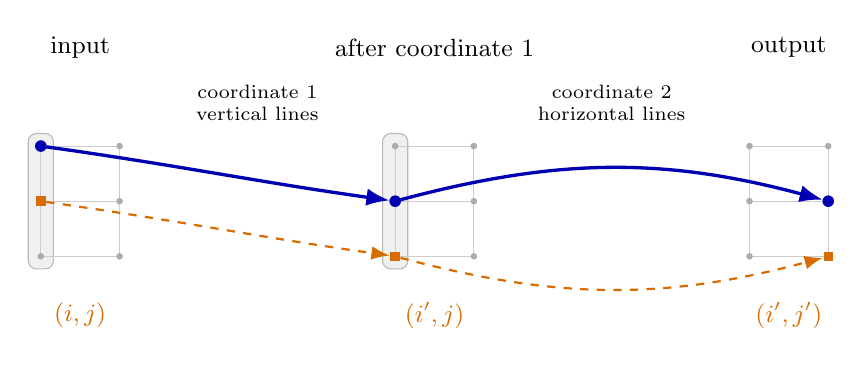
\begin{tikzpicture}[x=1cm,y=1cm,>=Latex]
\foreach \x in {0,4.5}{
 \path[fill=gray!12,draw=gray!55,rounded corners=3pt]
   ({\x-.16},-.16) rectangle ({\x+.16},1.56);
}
\foreach \x/\name in {0/{input},4.5/{after coordinate 1},9/{output}}{
 \node[font=\small] at ({\x+.5},2.65) {\name};
 \foreach \y in {0,.7,1.4}
   \draw[gray!40] (\x,\y)--({\x+1},\y);
 \foreach \dx in {0,1}
   \draw[gray!40] ({\x+\dx},0)--({\x+\dx},1.4);
 \foreach \y in {0,.7,1.4}
   \foreach \dx in {0,1}
     \fill[gray!65] ({\x+\dx},\y) circle (1.2pt);
}
\node[font=\scriptsize,align=center] at (2.75,1.95)
  {coordinate 1\\vertical lines};
\node[font=\scriptsize,align=center] at (7.25,1.95)
  {coordinate 2\\horizontal lines};

\draw[very thick,blue!70!black,->,shorten >=2pt,shorten <=2pt]
  (0,1.4) to[out=-8,in=172] (4.5,.7);
\draw[very thick,blue!70!black,->,shorten >=2pt,shorten <=2pt]
  (4.5,.7) to[out=15,in=165] (10,.7);
\draw[thick,dashed,orange!85!black,->,shorten >=2pt,shorten <=2pt]
  (0,.7) to[out=-8,in=172] (4.5,0);
\draw[thick,dashed,orange!85!black,->,shorten >=2pt,shorten <=2pt]
  (4.5,0) to[out=-15,in=195] (10,0);

\foreach \p in {(0,1.4),(4.5,.7),(10,.7)}
 \fill[blue!70!black] \p circle (2.1pt);
\foreach \p in {(0,.7),(4.5,0),(10,0)}
 \node[rectangle,fill=orange!85!black,inner sep=1.7pt] at \p {};
\node[font=\small,text=orange!85!black] at (.5,-.75) {$(i,j)$};
\node[font=\small,text=orange!85!black] at (5,-.75) {$(i',j)$};
\node[font=\small,text=orange!85!black] at (9.5,-.75) {$(i',j')$};
\end{tikzpicture}

\caption{Schematic of selected slots in three layers of a grid with two coordinates.
The first coordinate is drawn vertically and the second horizontally.
The solid prescribed path and dashed added path share the highlighted
line at the first stage but use distinct slots at every layer. The added path from
\((i,j)\) to \((i',j')\) must pass through \((i',j)\). On the shared line this
configuration has \(h_L=1\) and \(v_L=1\), illustrating how a prescribed
assignment reduces the slots available to an added path.}
\label{fig:trajectory}
\end{figure}

On a line used by the added paths, with \(m=|L|\) and \(v=v_L>0\), the
conditional probability is
\[
 \frac{L_m(z)(E_L(\mathcal H^+))}
      {L_m(z)(E_L(\mathcal H))}
 \le \frac4{(m-h_L)_v}.
\]
Indeed the corresponding uniform ratio is exactly \((m-h_L)_v^{-1}\);
\eqref{ac:eq:3} changes its numerator and denominator by factors between
\(1/2\) and \(2\). The uniform ratio records the increment of the line cost:
\[
 \frac1{(m-h_L)_v}
 =m^{-v}\exp\{\phi_m(h_L+v)-\phi_m(h_L)\}.
\]
Unused lines contribute one, and at most \(tb\) lines are used. Each added
path contributes \(\prod_jm_j^{-1}=s^{-1}\). Multiplying the line bounds gives
\begin{equation}
 p_{\mathcal H}(x,y)
 \le s^{-t}\exp\{C(\mathcal H^+)-C(\mathcal H)+(\log4)tb\}.
 \label{ac:eq:4}
\end{equation}
The difference of potentials is the part of this estimate that permits
further paths to be revealed during the induction.

For a positive integer \(q\) to be fixed, define the unnormalized Schatten
moment
\[
 T_\lambda^{\mathcal H}=\|K_\lambda^{\mathcal H}\|_{2q}^{2q}.
\]

\begin{samepage}
\begin{theorem}[Conditional sweep moment estimate]
There\label{thm:conditional}\label{ac:main} are a power of two \(R\ge2\), a positive integer \(q\), and \(z_*>0\) such
that every grid and every family \(\mathcal H\) of prescribed disjoint
trajectories defined above satisfy, for every \(z\in[0,z_*]\) and every
\(\lambda\vdash s-h\),
\begin{equation}
 \log T_\lambda^{\mathcal H}\ \le\
 -c(s)F(\lambda)+e(s)h\log s-C(\mathcal H).
 \label{ac:eq:15}
\end{equation}
Here a zero moment gives \(-\infty\). Use parameters
\[
 a=\frac1{100},\quad c_0=e_0=\frac a{100},\qquad
 c(s)=c_0+\frac1{\sqrt{\log s}},\qquad
 e(s)=e_0-\frac1{\sqrt{\log s}}.
\]
The empty diagram has dimension one. If \(h=s\), the remaining bijection is
the unique empty bijection and its moment is one. The assertion also includes
the one-dimensional trivial representation for every \(h\).
\end{theorem}
\end{samepage}

For \(\mathcal H=\varnothing\), the estimate is
\(T_\lambda^\varnothing\le D_\lambda^{-c(s)}\); Section~\ref{sec:analytic}
uses this estimate for small real parameters in the analytic transfer. For general
\(\mathcal H\), the term \(-C(\mathcal H)\) is retained because
\eqref{ac:eq:4} expresses the cost of prescribing additional paths as a difference of
potentials. Section~\ref{sec:induction} uses that difference to recover the
original potential after summing over the added placements.

\section{Contraction at sparse representation levels}\label{sec:sparse}
\label{ac:part:51}

We now contract an irreducible that first appears on a short list of cards,
even after a comparable number of trajectories has been prescribed. The row
case uses an alternating placement kernel. The column case uses the same
placement representation twisted by sign.

\begin{lemma}[Conditional sparse contraction]\label{lem:sparse}
For every \(0<\theta<1\) and \(K_0\ge1\), there are \(\rho>0\) and \(R_0\)
such that, for each power of two \(R\ge R_0\), one can choose
\(z_{\rm sp}(R)>0\) with the following property. For every allowed grid and
prescribed family \(\mathcal H\), suppose that the integer \(k\ge1\) satisfies
\begin{equation}
 h\le K_0 k,\qquad h+k\le s^{1-\theta},
 \label{ac:eq:5}
\end{equation}
and let \(\lambda\vdash M=s-h\) satisfy
\(\lambda_1=M-k\) or \(\lambda'_1=M-k\). Then, for every
\(z\in[0,z_{\rm sp}(R)]\),
\begin{equation}
 \|K_\lambda^{\mathcal H}\|_{\rm op}\le s^{-\rho k}.
 \label{ac:eq:6}
\end{equation}
\end{lemma}
\begin{proof}
Put \(B_0=\lceil8/\theta\rceil\). For \(b>B_0\) we use only the line comparison
\eqref{ac:eq:3}. For \(b\le B_0\) we first prove the estimate at \(z=0\), then
use continuity after fixing \(R\). The implicit constants in the entry
estimates below are absolute; their absorption into powers of \(s\) will
determine how large \(R\) must be in terms of \(\theta,K_0\).

First assume \(\lambda_1=M-k\). For input and output \(k\)-placements \(x,y\),
let \(p_A(x_A,y_A)\) be the conditional probability of the paths for the
labels in \(A\subseteq[k]\), with \(p_\varnothing=1\). Define a kernel from
input placements to output placements by
\begin{equation}
 Q(x,y)=s^{-k}\sum_{A\subseteq[k]}(-1)^{k-|A|}s^{|A|}p_A(x_A,y_A).
 \label{ac:eq:7}
\end{equation}
Its \(A=[k]\) term is the full placement transition kernel. For a proper
subset \(A\), the corresponding operator has output range among the
pullbacks \(y\mapsto f(y_A)\) of functions on \(|A|\)-placements. This
subrepresentation contains only types with first row at least
\(M-|A|>M-k\), by the branching rule in Section~\ref{sec:prelim}. Projection
to type \(\lambda\) therefore kills every term for a proper subset. The full
placement representation contains \([\lambda]\), so its surviving block is a
copy of \(K_\lambda^{\mathcal H}\). Consequently
\(\|K_\lambda^{\mathcal H}\|_{\rm op}\le\|Q\|_{\rm HS}\).
The scale \(s\) in \eqref{ac:eq:7} will cancel the probability \(1/s\) of a
path whose stage lines are untouched by every other constraint.

If the paths of \(A\) augment \(\mathcal H\) to a disjoint family
\(\mathcal H_A\), then \eqref{ac:eq:4} and
\(C(\mathcal H_A)\le b(h+|A|)\) give a crude bound. Invalid subsets have
probability zero. Summing over \(A\) yields
\begin{equation}
 |s^kQ(x,y)|\le 2^k\exp\{bh+(1+\log4)bk\}.
 \label{ac:eq:8}
\end{equation}

To count these entries, extend \(Q\) by zero when either endpoint array fails
to be an injection into its available input or output slots. On endpoint
placements we keep the alternating formula \eqref{ac:eq:7}, even when the
full family of \(k\) paths collides at an intermediate layer. Now choose all
input and output slots independently and uniformly from the full grid
\(\Omega\), with replacement. The zero extension gives the exact identity
\[
 \|Q\|_{\rm HS}^2
 =s^{-2k}\sum_{x,y\in\Omega^k}|s^kQ(x,y)|^2
 =\mathbb E_{\rm full}|s^kQ(x,y)|^2.
\]
Every sampled pair of endpoints determines an auxiliary trajectory by the
layer formula in Section~\ref{sec:paths}. At any fixed layer its slot is
uniform in \(\Omega\), and the slots for different particles are independent.
The following counting estimates use this independence between particles;
the conditional shuffle probabilities remain inside \(Q\).

We will count two kinds of sharing: a common slot at a layer, or a common line
at a stage. Suppose \(\omega\) bounds the probability that one independent
particle shares with any fixed trajectory. Form the graph whose vertices are
the particles and holes, with an edge for each sharing involving a particle.
For \(0\le w\le k\), if at least \(w\) particles are incident to edges, this graph contains a
directed forest with at least \(\lceil w/2\rceil\) edges and distinct particle
tails. To see this, in a component meeting holes, point each particle to a
neighbor one step closer to the nearest hole. Distances decrease along these
edges, so they form a forest rooted at holes, with every particle a tail. In
a component containing only particles, with \(v\ge2\) incident vertices, a rooted spanning
tree supplies \(v-1\ge v/2\) particle tails.

For a fixed directed forest with \(j\) edges, condition on all paths except a
leaf particle. Its parent is now fixed, its sharing event has probability at
most \(\omega\), and it occurs in no other remaining edge. Removing leaves
one by one bounds the forest probability by \(\omega^j\). There are at most
\(\binom{k}{j}(k+h)^j\) choices of its tails and parents. Thus, if
\(r=(k+h)\omega\le1\), the probability that at least \(w\) particles are
incident to sharing is at most
\begin{equation}
 \sum_{j=\lceil w/2\rceil}^{k}\binom{k}{j}r^j
 \le 2^k r^{w/2}.
 \label{ac:eq:9}
\end{equation}

For \(b>B_0\), take sharing to mean a common stage line. A particle uses a
fixed line at stage \(j\) with probability \(m_j/s\), so
\(\omega\le b\max_jm_j/s\). Since \(\max_jm_j\le s^{2/b}\),
\[
 (k+h)\omega\le b\,s^{-\theta+2/b}\le s^{-\theta/2}
\]
for sufficiently large \(R\), uniformly in \(b>B_0\). Here \(2/b<\theta/4\),
and \(b\le s^{\theta/4}\) follows uniformly from \(s\ge R^b\) after increasing
\(R\).

If a path shares no stage line with another particle path or a hole, adding
it to any subset multiplies that subset's transition probability by \(1/s\).
Its lines are independent of all the other constraints, and each uses the
uniform marginal for one slot. The statement also holds when the subset has
probability zero. The paired terms in \eqref{ac:eq:7} therefore cancel.
Thus \(Q\ne0\) requires all \(k\) particles to be incident to line sharing.
Using \eqref{ac:eq:9} with \(w=k\) and then \eqref{ac:eq:8},
\[
\begin{aligned}
 \Pr_{\rm full}(Q\ne0)&\le2^k s^{-\theta k/4},\\
 \|Q\|_{\rm HS}
 &\le2^{3k/2}e^{bh+(1+\log4)bk}s^{-\theta k/8}
 \le s^{-\theta k/16}
\end{aligned}
\]
for large \(R\). The last step uses \(h\le K_0k\) and
\(b/\log s\le1/\log R\).

\subsection{A bounded number of coordinates}
\label{ac:part:85}
When \(b\le B_0\), a line can occupy a substantial fraction of the grid, so
many paths may share a line. We work at \(z=0\) and use the fact that most
paths still see only a small fraction of each line prescribed. Put
\[
 \xi=\frac1{10B_0},\qquad \eta=s^{-\xi},
\]
and increase \(R\) so that \(\eta\le1/2\) for all \(s\ge R\).

For any endpoint arrays, let \(t_L\) be the number of their \(k\) auxiliary
paths using line \(L\), whether or not those paths are jointly feasible. Call
\(L\) light if \(h_L+t_L\le |L|\eta\). A particle is good if every line on its
path is light and it shares no slot at any layer with another particle or a
hole. Let \(G\) be the set of good particles. We first prove the entry bound
\begin{equation}
 |s^kQ|\le \exp(O(b(k+h)))\,\eta^{|G|/2}.
 \label{ac:eq:10}
\end{equation}
It is immediate for the zero extension outside endpoint placements, so
consider an entry of the original placement matrix. For a subset \(A\) whose
paths are compatible with \(\mathcal H\) at every layer, the uniform
conditional line law gives
\[
 s^{|A|}p_A(x_A,y_A)
 =\prod_L\frac{m^{v_L(A)}}{(m-h_L)_{v_L(A)}},
 \qquad m=|L|,
\]
where \(v_L(A)\) counts its paths on \(L\). For an invalid subset \(A\), its
probability is zero and this product is not formed.

Because a good path shares no layer slot with another path or a hole,
\(J\cup S\) is valid exactly when \(J\) is valid for every
\(J\subseteq[k]\setminus G\) and \(S\subseteq G\). We may therefore group the
alternating sum by \(J\) and discard every invalid \(J\) before forming line
factors. For a valid \(J\), let \(r_L(J)\) count its paths on \(L\), and
define
\[
 D_J=\prod_{L\text{ non-light}}
       \frac{m^{r_L(J)}}{(m-h_L)_{r_L(J)}},\qquad m=|L|.
\]
All these denominators are positive. The bound for \(\phi_m\) in
Section~\ref{sec:paths} gives
\[
\begin{aligned}
 \log D_J
 &=\sum_{L\text{ non-light}}
    \bigl(\phi_{|L|}(h_L+r_L(J))-\phi_{|L|}(h_L)\bigr)
 \\
 &\le\sum_L\phi_{|L|}(h_L+r_L(J))
 \le b(h+|J|).
\end{aligned}
\]

At each light line introduce \(W_L=m/Z_L\), where the \(Z_L\) are independent
gamma variables with shape \(m-h_L+1\) and unit rate. The elementary identity
\[
 \mathbb E Z^{-v}=\frac{\Gamma(\alpha-v)}{\Gamma(\alpha)}
 \quad\text{for }Z\sim\operatorname{Gamma}(\alpha,1),\quad 0\le v<\alpha,
\]
follows by integrating the gamma density. It gives
\(\mathbb E W_L^v=m^v/(m-h_L)_v\) for the exponents used here. Lightness makes
these moments finite. If \(L_j(i)\) denotes the stage-\(j\) line of a good
path \(i\), alternation over the good paths now gives the exact expression
\[
\begin{split}
 s^kQ(x,y)
 =\sum_{\substack{J\subseteq[k]\setminus G\\J\text{ valid}}}
 &(-1)^{k-|J|-|G|}D_J\\
 &\times\mathbb E\!\left[
   \prod_{L\text{ light}}W_L^{r_L(J)}
   \prod_{i\in G}\left(\prod_{j=1}^bW_{L_j(i)}-1\right)\right].
\end{split}
\]
Every path using a light line uses the same variable \(W_L\). We will group all
factors by line before taking moments; independence is available between
lines, not between particle factors.

For nonnegative integers \(u,v\) with \(u+v\le t_L\), density tilting gives
\begin{equation}
 \mathbb E W_L^v|W_L-1|^u
 =\frac{m^{u+v}}{(m-h_L)_{u+v}}\,
       \mathbb E|1-Z'/m|^u
 \le C_1^{u+v}\eta^{u/2},
 \label{ac:eq:11}
\end{equation}
where \(Z'\) has gamma shape \(n=m-h_L+1-u-v\) and unit rate, and \(C_1\) is absolute.
Indeed lightness gives the margin
\[
 n\ge m(1-\eta)+1>0,\qquad
 \frac{m^{u+v}}{(m-h_L)_{u+v}}
 \le(1-\eta)^{-(u+v)}\le2^{u+v}.
\]
For a gamma variable of shape \(n\), the centered moment generating function
is \(e^{-nt}(1-t)^{-n}\); its logarithm is at most \(Cnt^2\) for
\(|t|\le1/2\). Chernoff's inequality gives
\(\Pr(|Z'-n|>x)\le2\exp[-c\min\{x^2/n,x\}]\). Integrating this tail yields
\[
 (\mathbb E|Z'-n|^u)^{1/u}\le C(\sqrt{nu}+u),\qquad u\ge1.
\]
When \(u\ge1\), we have \(u/m\le\eta\), \(n\le m+1\), and
\(\lvert1-n/m\rvert\le\eta+1/m\le2\eta\), since \(1\le u\le m\eta\).
The triangle inequality therefore gives
\[
 (\mathbb E|1-Z'/m|^u)^{1/u}
 \le |1-n/m|+\frac C m(\sqrt{nu}+u)
 \le C'\sqrt\eta.
\]
This proves \eqref{ac:eq:11}; when \(u=0\), only the prefactor bound is needed.

For each good path, telescope in stage order:
\[
 \prod_{j=1}^bW_{L_j(i)}-1
 =\sum_{a=1}^b (W_{L_a(i)}-1)\prod_{j<a}W_{L_j(i)}.
\]
In one expanded term, let \(u_L\) count its factors \(W_L-1\), and \(v_L\)
its undifferenced factors \(W_L\). Each good path supplies one difference,
so \(\sum_Lu_L=|G|\). A tracked path supplies at most one factor at any
line at a given stage, so \(u_L+v_L\le t_L\). Independence across lines and
\eqref{ac:eq:11} bound the expectation of that term in absolute value by
\(C_1^{bk}\eta^{|G|/2}\). There are at most \(b^{|G|}\) telescoping choices
and \(2^{k-|G|}\) choices of valid \(J\). Together with the bound on \(D_J\),
these prove \eqref{ac:eq:10}.

It remains to count good particles. All probabilities in this count again
refer to the independent endpoint arrays sampled with replacement in the full grid;
the holes are fixed. The sparse hypothesis and
\(\xi=1/(10B_0)\le\theta/80\) give, for large \(R\),
\[
 \frac{(b+1)(k+h)}s\le s^{-\theta/2},\qquad
 \frac{2h}{s\eta},\ \frac{2k}{s\eta}
 \le2s^{-(\theta-\xi)}\le s^{-\theta/2}.
\]
In particular these quantities are at most one.

If \(|G|<k/2\), either at least \(k/4\) particles share a layer slot with
another path, or at least \(k/4\) particles use a non-light line. The first
event is bounded by \eqref{ac:eq:9} with \(\omega=(b+1)/s\). In the second
event, some stage \(j\) has at least \(k/(4B_0)\) particles on non-light
lines. Each such line satisfies \(h_L>m_j\eta/2\) or \(t_L>m_j\eta/2\), so
one of these two classes receives at least
\(a_k=k/(8B_0)\) particles.

At a fixed stage, the lines with \(h_L>m_j\eta/2\) are determined by the
holes and occupy a fraction at most \(2h/(s\eta)\) of the slots. The
independent occupancy bound for at least \(a_k\) particles in this fixed set
is \(2^k(2h/(s\eta))^{a_k}\). For the lines with \(t_L>m_j\eta/2\), their
number is at most \(r_j=\lfloor2k/(m_j\eta)\rfloor\). If \(r_j=0\), there
are none. Otherwise fix a set of at most \(r_j\) lines first. A particle
uses it with probability at most \(r_jm_j/s\le2k/(s\eta)\), so its occupancy
bound is \(2^k(2k/(s\eta))^{a_k}\). We then sum over the at most
\((s+1)^{r_j}\) possible fixed sets. Combining the three events gives
\[
\begin{split}
 \Pr_{\rm full}(|G|<k/2)\le {}&
 2^k\left(\frac{(b+1)(k+h)}s\right)^{k/8}
 +b\,2^k\left(\frac{2h}{s\eta}\right)^{a_k}\\
 &+2^k\sum_{\substack{1\le j\le b\\r_j\ge1}}
       (s+1)^{r_j}\left(\frac{2k}{s\eta}\right)^{a_k}.
\end{split}
\]
The thresholds may be nonintegral: taking their ceilings only decreases
these powers of bases in \([0,1]\).

The cost of choosing the lines with \(t_L>m_j\eta/2\) is uniformly small. Since
\(b\le B_0\) and \(R\le m_j\le R^2\),
\[
 m_j\ge s^{1/(2B_0)},\qquad m_j\eta\ge s^{2/(5B_0)},\qquad
 \frac{r_j\log(s+1)}{k\log s}
 \le2s^{-2/(5B_0)}\frac{\log(s+1)}{\log s}=o_R(1).
\]
Before the factors \(2^k\), the stage sum, and this set count, the vertex
term saves \((\theta/16)k\log s\) and each term for non-light lines saves
\((\theta/(16B_0))k\log s\). The displayed ratio tends to zero uniformly for
\(s\ge R\); the other two factors also cost \(o_R(k\log s)\). Increasing
\(R\) therefore gives
\begin{equation}
 \Pr_{\rm full}(|G|<k/2)\le s^{-\nu k},
 \qquad \nu=\frac{\theta}{100B_0}>0,
 \label{ac:eq:12}
\end{equation}
uniformly over the grids with \(b\le B_0\). On \(|G|\ge k/2\),
\eqref{ac:eq:10} gives the entry saving \(s^{-\xi k/4}\). On the complement,
use \eqref{ac:eq:8} and the square root of \eqref{ac:eq:12} in the
Hilbert--Schmidt expectation. We obtain
\[
 \|Q\|_{\rm HS}
 \le \exp(O(b(k+h)))
       \left(s^{-\xi k/4}+s^{-\nu k/2}\right).
\]

\subsection{Column types and the common perturbation interval}

Suppose now that \(\lambda'_1=M-k\). The sign twist of the \(k\)-placement
representation contains \([\lambda]\). Its entry for placements \(x,y\) is
the conditional average of
\(\operatorname{sgn}(g)\mathbf1_{\{g(x)=y\}}\), where \(g\) is the remaining
bijection in fixed slot identifications. An entry whose full path family is
invalid is zero. For a valid entry, condition on all \(h+k\) paths.

On each line, list the assigned paths first in the same order at input and
output, followed by the unassigned sites. Deleting the fixed assignments
then leaves a residual bijection, and comparison with the original slot
orders contributes only a deterministic sign. Applying this to the lines and
composing the stages expresses the sign of the remaining bijection as a fixed
factor times the product of the residual line signs. The conditioned lines
are independent. It is therefore enough to find one line whose residual sign
has mean zero.

For \(b>B_0\),
\[
 \frac{s}{\max_jm_j}\ge s^{1-2/b}>s^{1-\theta}\ge h+k.
\]
Every stage has more lines than paths, so it has a line untouched by all
\(h+k\) paths. Its residual law is \(L_m(z)\), which has expected sign zero.
For \(b\le B_0\) at \(z=0\), fix any stage \(j\). The number of unassigned
sites satisfies
\[
 s-h-k\ge s(1-s^{-\theta})>\frac{s}{m_j}
\]
once \(R^{-\theta}+R^{-1}<1\). There are \(s/m_j\) lines in that stage, so one
line has at least two unassigned sites. Its residual bijection under the
uniform conditional law is uniform between the unassigned site sets and has expected sign
zero. Thus every signed placement entry vanishes in the relevant parameter
range of each branch.

We finish by fixing the constants in the promised order. Set
\(\beta=\min\{\xi/4,\nu/2\}>0\). For an absolute constant \(C\), the
bounded-coordinate row estimate is at most
\[
 2e^{Cb(1+K_0)k}s^{-\beta k}\le s^{-\beta k/2}
\]
for all sufficiently large \(R\), since \(b/\log s\le1/\log R\).
The corresponding
column operator is zero at \(z=0\). The many-coordinate row estimate is
at most \(s^{-\theta k/16}\), and its column operator is zero whenever
\eqref{ac:eq:3} holds. We may therefore choose
\[
 \rho=\min\{\theta/32,\beta/4\}>0
\]
before \(R\), then choose \(R_0\) large enough for all the preceding estimates.
For every \(R\ge R_0\), the bounded-coordinate bounds at \(z=0\) have strict
slack relative to \(s^{-\rho k}\).

Fix now a power of two \(R\ge R_0\). When \(b\le B_0\), there are finitely
many allowed grids, with \(s\le R^{2B_0}\), and finitely many feasible path
families, integers \(k\), and partitions. Each conditional operator is a
finite expression in line probabilities whose conditioning denominators are
positive at \(z=0\); it is therefore continuous there. Strict slack and
finiteness give \(\delta(R)>0\) such that \eqref{ac:eq:6} holds for all these
bounded-coordinate operators when \(0\le z\le\delta(R)\). Set
\[
 z_{\rm sp}(R)=\min\{\delta(R),z_{\rm cmp}(R)\}>0.
\]
The many-coordinate proof applies throughout this interval by
\eqref{ac:eq:3}, so it covers every \(b\) and completes the lemma.
\end{proof}

\section{Positive tensor densities for hook diagrams}\label{sec:density}
\label{ac:part:120}

The sparse estimate settles small representation dimensions. For the
remaining diagrams, the induction will compare row and column symmetry on
a rectangle with holes. We construct positive tensor densities that
dominate the projections for hook diagrams. Their trace-one normalization
will permit that comparison even after sites have been removed.

Let \(p\in[1,s]\) be an integer and let \(V=E\oplus O\), where \(E\) and
\(O\) each have dimension \(p\). On \(V^{\otimes l}\), \(l\le s\), let
\(S_l\) permute the slots with signs: interchanging two neighboring odd
factors (vectors in \(O\)) incurs a minus sign, and the other neighboring
interchanges do not. On parity-homogeneous tensors the sign is therefore
the sign of the induced reordering of the odd factors. This defines a
unitary action. An \emph{even density} is a positive semidefinite operator
on \(V\) of trace one that is block diagonal for \(E\oplus O\).

\begin{lemma}[Signed density domination]\label{lem:density}
Let \(P_\alpha\) be the isotypic projection for \(\alpha\vdash l\) in this
signed tensor representation. The types present are precisely those in the
\((p,p)\)-hook: all their boxes lie in the first \(p\) rows or the first
\(p\) columns. For every such type there is a probability distribution
\(\mu_\alpha\) on even densities such that, in positive semidefinite order,
\begin{equation}
 P_\alpha\preceq
 \exp\{F(\alpha)+O(p^2\log(s+1))\}
 \mathbb E_{r\sim\mu_\alpha}r^{\otimes l}.
 \label{ac:eq:13}
\end{equation}
Its multiplicity is at most \(\exp(O(p^2\log(s+1)))\), and the number of
types present is at most \((s+1)^{2p}\). All constants are absolute.
\end{lemma}

The signed tensor action and its hook support are classical in the hook
theory of Berele and Regev~\cite{BereleRegev1983}. Positive domination by
mixtures of tensor powers also underlies the postselection technique of
Christandl, K\"onig and Renner~\cite{ChristandlKonigRenner2009}. We derive
the needed signed form from ordinary Schur--Weyl sectors, keeping the
irreducible dimension \(D_\alpha\) explicit.

\begin{proof}
For \(l=0\), the tensor space and its only representation have dimension
one, and any density gives the assertion. Suppose \(l>0\). Fix the number
\(t\) of even factors. A fixed parity pattern has the ordinary tensor
powers of \(E\) and \(O\), with the symmetric-group action on the latter
twisted by sign. Summing over parity patterns induces this action from
\(S_t\times S_{l-t}\) to \(S_l\). Write \(W_\sigma(E)\) and \(W_\tau(O)\)
for the ordinary Schur--Weyl multiplicity spaces, the polynomial
irreducibles of highest weights \(\sigma\) and \(\tau\). The resulting
orthogonal sectors, indexed by \(\sigma\vdash t\) and \(\tau\vdash l-t\)
with at most \(p\) rows each, are
\[
 \mathcal V_{\sigma,\tau}\cong
 \operatorname{Ind}_{S_t\times S_{l-t}}^{S_l}
       ([\sigma]\boxtimes[\tau'])
 \otimes W_\sigma(E)\otimes W_\tau(O).
\]
This decomposition records the commuting actions of \(S_l\) and
\(U(E)\times U(O)\): the induction records the positions of the two
parities, and the transpose on \(\tau\) records the odd sign twist.

The representation \([\tau']\) occurs upon inducing sign representations
on subgroups of sizes \(\tau_1,\ldots,\tau_p\), since its columns can be
added successively as vertical strips. Thus, if \(\alpha\) occurs in
\(\mathcal V_{\sigma,\tau}\), Pieri's rule reaches it from \(\sigma\) by
at most \(p\) vertical strips. Transposing and interchanging the two
factors gives the analogous statement starting from \(\tau\). Padding by
zeros,
\[
 \alpha_i\le\sigma_i+p,\qquad \alpha'_j\le\tau_j+p.
\]
In particular \(\alpha_{p+1}\le p\), the hook condition. Conversely, for
a hook shape take its first \(p\) rows as the even shape, then add its boxes
below those rows by columns from left to right. These are at most \(p\)
vertical strips. In the odd tensor power, words with one basis symbol for
each strip and with its prescribed multiplicity carry the corresponding
induction of sign representations. Pieri's rule therefore supplies the
given hook shape. The first \(p\) row lengths and first \(p\) column
lengths specify any hook shape, so there are at most \((s+1)^{2p}\) of
them.

We next compare the weight of a sector with the dimension of any type
\(\alpha\) occurring there. Put
\[
 \mathcal S=l\log l-\sum_i\sigma_i\log\sigma_i-\sum_j\tau_j\log\tau_j,
\]
with zero summands interpreted as zero. The horizontal and vertical arm
lengths of \(\alpha\) outside its \(p\)-by-\(p\) core are
\[
 H_i=(\alpha_i-p)_+\quad(i\le p),\qquad
 V_j=(\alpha'_j-p)_+\quad(j\le p).
\]
The strip inequalities give \(H_i\le\sigma_i\) and \(V_j\le\tau_j\).
Each hook in a horizontal arm is at most its row hook plus \(p\).
Consequently an arm of length \(H_i\) has hook product at most
\[
 \prod_{r=1}^{H_i}(r+p)
 =H_i!\binom{H_i+p}{p}
 \le H_i!(s+p)^p.
\]
The same bound holds for each vertical arm, and the at most \(p^2\) core
hooks have length at most \(s\). The hook-length formula now gives
\[
 D_\alpha\ge(s+p)^{-O(p^2)}
       \frac{l!}{\prod_i\sigma_i!\prod_j\tau_j!}.
\]
Using \(\log(n!)=n\log n-n+O(\log(n+1))\), whose linear terms cancel
because \(|\sigma|+|\tau|=l\), proves
\begin{equation}
 \mathcal S\le F(\alpha)+O(p^2\log(s+1)).
 \label{ac:eq:14}
\end{equation}

To obtain a positive density for the sector, define
\[
 d_E=\operatorname{diag}(\sigma_1/l,\ldots,\sigma_p/l),\qquad
 d_O=\operatorname{diag}(\tau_1/l,\ldots,\tau_p/l),
\]
and let \(r_U=(U_Ed_EU_E^*)\oplus(U_Od_OU_O^*)\), with independent Haar
unitaries on \(E\) and \(O\). This is an even density. Write
\(m_\sigma=\dim W_\sigma(E)\) and \(m_\tau=\dim W_\tau(O)\). The Weyl
dimension formula gives, for \(|\sigma|=t\),
\[
 m_\sigma
 =\prod_{1\le i<j\le p}
       \frac{\sigma_i-\sigma_j+j-i}{j-i}
 \le(t+1)^{p(p-1)/2},
\]
and the analogous bound for \(m_\tau\), with \(t\) replaced by \(l-t\).
The tensor power of \(d_E\) is positive and acts on the multiplicity
space as \(W_\sigma(d_E)\). Its highest-weight line has eigenvalue
\(\prod_i(\sigma_i/l)^{\sigma_i}\); all other eigenvalues are
nonnegative. The analogous statement holds for \(d_O\). These assertions
extend to zero eigenvalues by continuity, with \(0^0=1\).

The tensor density preserves every Schur--Weyl sector. Averaging over the
two unitary groups makes its action scalar on the two irreducible
multiplicity spaces. On the whole sector \(\mathcal V_{\sigma,\tau}\) the
scalar is
\[
 \frac{\Tr W_\sigma(d_E)}{m_\sigma}
 \frac{\Tr W_\tau(d_O)}{m_\tau}
 \ \ge\
 \frac{\prod_i(\sigma_i/l)^{\sigma_i}
       \prod_j(\tau_j/l)^{\tau_j}}{m_\sigma m_\tau}
 =\frac{e^{-\mathcal S}}{m_\sigma m_\tau}
 \ge e^{-\mathcal S-O(p^2\log(s+1))}.
\]
The same scalar acts on every parity pattern: the density preserves those
patterns and has the same tensor factors on each. Thus their number does
not enter the scalar. If \(Q_{\sigma,\tau}\) is the orthogonal projection
onto this sector, positivity and \eqref{ac:eq:14} give
\[
 Q_{\sigma,\tau}\preceq
 \exp\{F(\alpha)+O(p^2\log(s+1))\}\,\mathbb E_U r_U^{\otimes l}
\]
whenever \(\alpha\) occurs there.

The relevant sector projections cover \(P_\alpha\). Their number
\(N_\alpha\) is at most \((s+1)^{2p}\), because the two padded partitions
are specified by \(2p\) integers between zero and \(s\). Sum the last
bound over these sectors, and choose a sector uniformly before choosing
its two Haar unitaries. The resulting probability distribution
\(\mu_\alpha\) satisfies
\[
 \sum_{\text{relevant sectors}}\mathbb E_U r_U^{\otimes l}
 =N_\alpha\,\mathbb E_{r\sim\mu_\alpha}r^{\otimes l}.
\]
The factor \(N_\alpha\) is absorbed by \(O(p^2\log(s+1))\), proving
\eqref{ac:eq:13}. Finally, taking traces proves the multiplicity bound:
\(\Tr P_\alpha=D_\alpha\operatorname{mult}(\alpha)\), while every tensor
density has trace one.
\end{proof}

When sites are partitioned into blocks, signed unitary reordering makes
the action of their product subgroup a tensor product. Applying
\eqref{ac:eq:13} in each block therefore gives products of densities
constant within the blocks. Each density is even, so undoing the signed
reordering carries this to the ordinary tensor product with its sites
relabeled. In particular, a constant tensor power of an even density
commutes with the full signed symmetric-group action.

\section{The conditional moment induction}\label{sec:induction}
\label{ac:part:148}


We prove Theorem~\ref{thm:conditional} by induction on the number \(b\)
of coordinates, simultaneously for every allowed grid, path family, and
representation. First fix the constants in the order required by the
sparse estimate. Take \(\theta=a/16\) and \(K_0=10/e_0\) in
Lemma~\ref{lem:sparse}. Its exponent \(\rho\) is uniform for sufficiently
large \(R\), so we may next choose an integer
\[
 q\ge\max\{1,\lceil2/\rho\rceil\},\qquad 2q\rho\ge4,
\]
and only then choose a sufficiently large power of two \(R\). Every
largeness requirement below will hold uniformly for \(s\ge R\). In
particular, require
\[
 \frac1{\sqrt{\log R}}\le\frac{e_0}{2},
 \qquad
 \frac1{\log R}\le\frac{e_0}{4}.
\]
Since \(b\le\log s/\log R\) and \(C(\mathcal H)\le bh\), these choices give
\[
 c(s)\le2c_0,\qquad e(s)\ge e_0/2,\qquad
 e(s)h\log s-C(\mathcal H)\ge(e_0/4)h\log s.
\]
Further increases of \(R\) will absorb the displayed errors below.
After \(R\) is fixed, choose \(z_*>0\) small enough for
\eqref{ac:eq:3}, Lemma~\ref{lem:sparse}, and the base case.

Every conditional average is a contraction. Thus when \(F(\lambda)=0\),
its moment is at most one and the nonnegative allowance above proves the
theorem. This covers the empty diagram, \(M=1\), and all one-dimensional
types. A zero moment satisfies the bound by the convention
\(\log0=-\infty\).

For \(b=1\) and \(z=0\), conditioning on the prescribed assignments
leaves a uniform bijection of the remaining slots. Every nontrivial
average is therefore zero. Once \(R\) is fixed there are only finitely
many one-coordinate grids, path families, and representations, and their
conditional operators are continuous at zero. Decreasing \(z_*\) gives
the base case on a common interval.

Now assume \(b\ge2\) and the theorem for fewer coordinates. The contraction
bound gives \(T_\lambda^{\mathcal H}\le D_\lambda\), so the desired
inequality is automatic whenever
\begin{equation}
 (1+c(s))F(\lambda)\le e(s)h\log s-C(\mathcal H).
 \label{ac:eq:16}
\end{equation}
Suppose \(F(\lambda)<s^{1-a/4}\) and \eqref{ac:eq:16} fails. The positive
allowance above then gives
\(h\log s\le K_0F(\lambda)\), and \(M=s-h\ge s/2\) for large \(R\).
Put \(k=\min(M-\lambda_1,M-\lambda'_1)\). The dimension estimates from
Section~\ref{sec:prelim} give
\(c_{\rm dim}k\le F(\lambda)\le k\log s\). Hence \(h\le K_0k\), and
\[
 h+k\le s^{1-\theta}
\]
for large \(R\), because \(\theta=a/16<a/4\). Also \(k\ge1\), since
\(F(\lambda)>0\). Lemma~\ref{lem:sparse} applies. There are
\(D_\lambda\) singular values, so
\[
 \log T_\lambda^{\mathcal H}
 \le F(\lambda)-2q\rho k\log s
 \le-3F(\lambda)
 \le-c(s)F(\lambda)+e(s)h\log s-C(\mathcal H).
\]
This settles the sparse-dimension range.

We are left with \(b\ge2\) and the large-dimension range
\begin{equation}
 F(\lambda)\ge s^{1-a/4}.
 \label{ac:eq:17}
\end{equation}

\subsection{The hook estimate on the current grid}
\label{ac:part:199}

Removing the boxes outside a hook will record extra card trajectories.
We therefore first prove an estimate that is uniform over the resulting
path families. Set
\[
 p=\lfloor s^a\rfloor,\qquad
 \widehat c=c(s)+\frac{1}{20\sqrt{\log s}},\qquad
 \widehat e=e(s)-\frac{1}{20\sqrt{\log s}}.
\]
Under the induction hypothesis for fewer than \(b\) coordinates, we claim
that every family \(\mathcal H'\) of \(h'\) prescribed trajectories on
the current grid, with distinct slots at every layer and satisfying the
coordinate rule of Section~\ref{sec:paths}, and every \((p,p)\)-hook
diagram \(\gamma\vdash s-h'\), satisfy
\begin{equation}
 \log T_\gamma^{\mathcal H'}
 \le-\widehat c F(\gamma)+\widehat e h'\log s
       -C(\mathcal H')+s^{9/10}.
 \label{ac:eq:21}
\end{equation}
There is no lower bound on \(F(\gamma)\) in this claim. It retains the full
trajectory potential and improves both coefficients slightly. We will
derive it from two shorter coordinate sweeps, then use its dimension
reserve when the removed boxes are restored.

Split the coordinate list into consecutive parts of \(\lfloor b/2\rfloor\)
and \(\lceil b/2\rceil\) coordinates, with products \(s_1\) and \(s_2\).
Each coordinate contributes between \(\log R\) and \(2\log R\), so
\[
 \frac15\log s\le\log s_u\le\frac45\log s
 \qquad(u=1,2).
\]
In particular \(p\le s_u\). Regard the grid as \(s_2\) rows of length
\(s_1\). The first part of the sweep acts within rows and the second
within columns. At their junction, the middle positions of \(\mathcal H'\)
are removed, leaving a fixed board of \(s-h'\) free sites. Splitting each
prescribed trajectory there gives the path constraints in each row and
each column.

Use the signed tensor representation of Section~\ref{sec:density} on the
free sites at each layer. Let \(X\) be the conditional row average from
the input layer to the junction, and \(Y\) the conditional column average
from the junction to the output. The row and column randomizations are
conditionally independent under the fixed path constraints, so \(YX\) is
the full conditional average. At the junction let \(P_\gamma\) be the
full-group isotypic projection, and let \(P_\alpha^R,P_\beta^C\) be the
row and column subgroup projections. Here \(\alpha_i\) partitions the
number of free sites in row \(i\), and \(\beta_j\) partitions the number
of free sites in column \(j\); a row or column with no free sites has the
empty type. The sums below range over the local types occurring in the
signed tensor representation. Put
\[
 F_R=\sum_iF(\alpha_i),\qquad F_C=\sum_jF(\beta_j).
\]
The full projection commutes with both subgroup projections. Bijections
between the layers intertwine their full isotypic projections. Thus,
under compatible unitary identifications, the restriction of
\(Y P_\gamma X\) from the input \(\gamma\)-isotypic space to the output
\(\gamma\)-isotypic space is \(K_\gamma^{\mathcal H'}\otimes I\), where
the identity acts on the tensor multiplicity space. The hook type occurs
by Lemma~\ref{lem:density}, so this multiplicity is at least one.
Inserting the subgroup decompositions at the junction gives
\begin{equation}
\begin{aligned}
 (T_\gamma^{\mathcal H'})^{1/(2q)}
 &\le\|Y P_\gamma X\|_{2q}\\
 &\le\sum_{\alpha,\beta}
  \|Y P_\beta^C\|_{2q}\,
  \|P_\beta^C P_\gamma P_\alpha^R\|_{\rm op}\,
  \|P_\alpha^R X\|_{2q}.
\end{aligned}
\label{ac:eq:20}
\end{equation}
The first inequality uses the unnormalized trace on at least one copy of
\(\gamma\). The second uses the triangle inequality and the product norm
inequality, followed by \(\|A\|_{\rm op}\le\|A\|_{2q}\) for an outer
factor. We now bound the two child moments and the middle overlap.

Ordering the free sites by rows at both ends of the first part makes
\(X=\bigotimes_i X_i\); signed unitary reordering justifies this tensor
product. Write \(\mathcal H_i\) for the path constraints in row \(i\)
and \(\operatorname{mult}(\alpha_i)\) for the tensor multiplicity. Then
\[
 \|P_\alpha^R X\|_{2q}^{2q}
 =\prod_i \operatorname{mult}(\alpha_i)T_{\alpha_i}^{\mathcal H_i}.
\]
The column formula is identical. Lemma~\ref{lem:density} bounds each
multiplicity by \(\exp(O(p^2\log(s+1)))\). Apply the induction hypothesis
to every local constrained sweep and put
\[
 c_*=\min_{u=1,2}c(s_u),\qquad
 e_*=\max_{u=1,2}e(s_u).
\]
Each stage line belongs to exactly one child subproblem, so their
potentials add to \(C(\mathcal H')\). Each part has \(h'\) prescribed
trajectories, and their size weights add as
\(\log s_1+\log s_2=\log s\). Hence
\begin{equation}
\begin{aligned}
 \log\!\left(
 \|P_\alpha^R X\|_{2q}^{2q}\|Y P_\beta^C\|_{2q}^{2q}
 \right)
 \le{}&-c_*(F_R+F_C)+e_*h'\log s-C(\mathcal H')\\
 &+O((s_1+s_2)p^2\log(s+1)).
\end{aligned}
\label{ac:eq:18}
\end{equation}

The middle factor in \eqref{ac:eq:20} depends only on the fixed free-site
board. Its estimate does not use the trajectory probabilities.

\begin{lemma}[Overlap at the junction]\label{lem:overlap}
For the row and column type lists on the free junction sites and the full
hook type \(\gamma\) defined above,
\begin{equation}
 \log\|P_\beta^C P_\gamma P_\alpha^R\|_{\rm op}^2
 \le F_R+F_C-F(\gamma)+h'
       +O((s_1+s_2)p^2\log(s+1)).
 \label{ac:eq:19}
\end{equation}
Here a zero norm has logarithm \(-\infty\), and the constant is absolute.
\end{lemma}
\begin{proof}
Since \(P_\gamma\) commutes with both subgroup projections,
\[
 \|P_\beta^C P_\gamma P_\alpha^R\|_{\rm op}^2
 \le\|P_\beta^C P_\gamma P_\alpha^R\|_{\rm HS}^2
 =\Tr(P_\alpha^R P_\beta^C P_\gamma).
\]
The product \(P_\beta^C P_\gamma\) is a positive projection. We may
therefore dominate \(P_\alpha^R\) inside this trace by
Lemma~\ref{lem:density}. Apart from the factor
\(\exp(F_R+O(s_2p^2\log(s+1)))\), this leaves a probability mixture
of product densities whose one-site matrix in row \(i\) is an even
density \(r_i\).

For one such row family, average over all \(s_2\) rows, including empty
ones. For \(0<\varepsilon<1\), put
\[
 \bar r=\frac1{s_2}\sum_i r_i,\qquad
 \bar r_\varepsilon=(1-\varepsilon)\bar r+\varepsilon I/\dim V,
 \qquad A_\varepsilon=\bar r_\varepsilon^{-1/2}.
\]
The regularized reference density is even. With \(n=s-h'\), the positive
operator \(B_\varepsilon=\bar r_\varepsilon^{\otimes n}\) has trace one
and commutes with the full signed group action. On the
\(\gamma\)-isotypic space it has the form \(I_{D_\gamma}\otimes B_\gamma\).
Every eigenvalue there is therefore counted at least \(D_\gamma\) times
in its trace, and
\[
 B_\varepsilon P_\gamma\preceq D_\gamma^{-1}P_\gamma.
\]
It also commutes with \(P_\beta^C\). Compress this inequality by that
projection, use \(P_\beta^C P_\gamma\preceq P_\beta^C\) on the right, and
conjugate by \(B_\varepsilon^{-1/2}\). The result is
\[
 P_\beta^C P_\gamma
 \preceq D_\gamma^{-1}
 A_\varepsilon^{\otimes n}P_\beta^C A_\varepsilon^{\otimes n}.
\]

Now dominate the column projection by its density mixture. Apart from
the corresponding factor
\(\exp(F_C+O(s_1p^2\log(s+1)))\), each resulting mixture integrand is
the tensor-product trace
\[
 \prod_{(i,j)\text{ free}}
 \operatorname{tr}(A_\varepsilon r_i A_\varepsilon v_j),
\]
where \(v_j\) is the even density for column \(j\). Each factor is
nonnegative: it equals
\(\|r_i^{1/2}A_\varepsilon v_j^{1/2}\|_{\rm HS}^2\).
For every column, summing these factors over all rows gives
\[
 \sum_i\operatorname{tr}(A_\varepsilon r_i A_\varepsilon v_j)
 =s_2\operatorname{tr}(A_\varepsilon\bar r A_\varepsilon v_j)
 \le\frac{s_2}{1-\varepsilon}.
\]
If the column is missing \(l<s_2\) sites, AM--GM on its \(s_2-l\)
retained sites bounds their product by
\[
 (1-\varepsilon)^{-(s_2-l)}
 \left(\frac{s_2}{s_2-l}\right)^{s_2-l}
 \le(1-\varepsilon)^{-(s_2-l)}e^l.
\]
If \(l=s_2\), the empty column contributes the empty product one.
There are \(h'\) missing sites in total. Multiplication over columns,
averaging the uniformly bounded integrands, and then letting
\(\varepsilon\downarrow0\) prove \eqref{ac:eq:19}.
\end{proof}

We now combine the two estimates. Write \(W\) for the right side of
\eqref{ac:eq:19}, including its error. Terms with zero middle factor in
\eqref{ac:eq:20} contribute nothing. For a nonzero middle factor, its norm
is at most one as well as satisfying \eqref{ac:eq:19}. Since
\(c_*\le2c_0<1\le q\),
\[
 q\log\|P_\beta^C P_\gamma P_\alpha^R\|_{\rm op}^2
 \le c_*\min(0,W)\le c_*W.
\]
Adding this to \eqref{ac:eq:18} cancels \(F_R+F_C\). The number of lists
of local hook types contributes only
\(O_q((s_1+s_2)p^2\log(s+1))\) when the sum in \eqref{ac:eq:20} is
raised to \(2q\). We obtain
\[
 \log T_\gamma^{\mathcal H'}
 \le-c_*F(\gamma)+e_*h'\log s-C(\mathcal H')
       +c_*h'+O_q((s_1+s_2)p^2\log(s+1)).
\]

The size split gives the reserves in the claimed coefficients. With
\(L=\log s\),
\[
 c_*-c(s)=e(s)-e_*
 \ge\frac{\sqrt5/2-1}{\sqrt L}
 >\frac1{10\sqrt L}.
\]
The hats use only \(1/(20\sqrt L)\) of each reserve. The remaining hole
reserve is at least \(h'\sqrt L/20\), which absorbs \(c_*h'\) for large
\(R\). Also
\[
 (s_1+s_2)p^2\log(s+1)
 \le2s^{4/5+2a}\log(s+1)=2s^{0.82}\log(s+1).
\]
For fixed \(q\), the corresponding \(O_q\) error is at most \(s^{9/10}\)
once \(R\) is large.
These comparisons prove \eqref{ac:eq:21} for every allowed
\(\mathcal H'\) and hook type, including the types of small dimension.

\subsection{Adding the cells outside the hook}
\label{ac:part:245}

Return to the diagram \(\lambda\) in \eqref{ac:eq:17}. Keep its
\((p,p)\)-hook part \(\gamma\), which is a Young diagram. Translate the
remaining boxes by subtracting \(p\) from both indices to obtain an
ordinary partition \(\delta\), and put \(k=|\delta|\). The skew shape
\(\lambda/\gamma\) is a translate of \(\delta\), so branching and
Frobenius reciprocity give multiplicity \(D_\delta\) for \(\lambda\) in the representation
induced from \([\gamma]\) on \(S_{M-k}\) to \(S_M\). That induced space has
dimension \((M)_kD_\gamma\). In particular,
\begin{equation}
 F(\lambda)\le F(\gamma)+k\log s.
 \label{ac:eq:22}
\end{equation}

Realize the induced space with one fiber of type \([\gamma]\) for each
placement of \(k\) distinguishable cards in the free slots. A bijection
moves the placement and acts on its fiber by the bijection of the
remaining slots; consistent identifications of those slot sets change
the fiber maps only by unitaries. The average block from placement \(x\)
to placement \(y\) is \(p_{\mathcal H}(x,y)\) times the conditional
operator in \([\gamma]\) after those extra trajectories have been
prescribed. If this probability is positive, the endpoints force a
feasible augmented family \(\mathcal H'\) of \(h+k\) trajectories.
Thus \eqref{ac:eq:21} applies to every nonzero block, with no dimension
condition on \(\gamma\).

The \(2q\)-moment of the induced average is the sum of the irreducible
moments with their multiplicities, and hence is at least
\(D_\delta T_\lambda^{\mathcal H}\). Expand its trace as a sum over
cyclic placement indices with \(2q\) edges, alternating between the
input and output placement sets. Let \(p_j\) be the transition entry on
edge \(j\), using the transposed transition matrix on an adjoint edge.
The fiber map on an adjoint edge is the adjoint of its corresponding
forward conditional operator. It has the same singular values and uses
the same forward path potential. For a nonzero cyclic term, write
\(\mathcal H'_j\) for these augmented paths on edge \(j\).
The triangle inequality and matrix trace H\"older give
\begin{equation}
 D_\delta T_\lambda^{\mathcal H}
 \le \sum
 \left(\prod_{j=1}^{2q}p_j\right)
 \prod_{j=1}^{2q}(T_\gamma^{\mathcal H'_j})^{1/(2q)}.
 \label{ac:eq:23}
\end{equation}
The sum may be restricted to nonzero cyclic terms.

Apply \eqref{ac:eq:21}. Apart from the potential
\(-C(\mathcal H'_j)\), its terms depend only on \(s,h+k,\gamma\), so the
same bound applies on every edge. To handle the potentials, apply
\eqref{ac:eq:4} to a \(1/(2q)\) power of each \(p_j\). Multiplication
over the edges yields
\[
 \prod_{j=1}^{2q}\left(p_j e^{-C(\mathcal H'_j)/(2q)}\right)
 \le s^{-k}\exp\{-C(\mathcal H)+(\log4)kb\}
       \prod_{j=1}^{2q}p_j^{1-1/(2q)}.
\]
The augmented potentials have disappeared, leaving the potential of the
original path family.

It remains to sum the last product. Put \(n_k=(M)_k\) and label the
\(2q\) placement variables \(x_1,\ldots,x_{2q}\) cyclically. Each edge
matrix is the placement transition matrix or its transpose. Both row
and column sums are one, because the transition averages bijections of
the free slots. For each \(r\), let \(A_r\) be the product of all edge
entries except the \(r\)th. Then
\[
 \prod_{j=1}^{2q}p_j^{1-1/(2q)}
 =\prod_{r=1}^{2q}A_r^{1/(2q)}.
\]
Deleting an edge opens the cycle into a chain. Successive summation over
an endpoint of that chain uses a row or column sum equal to one; the
last placement has \(n_k\) possible values. Hence \(\sum A_r=n_k\)
for every \(r\), and scalar H\"older gives
\[
 \sum_{x_1,\ldots,x_{2q}}\prod_{j=1}^{2q}p_j^{1-1/(2q)}
 \le\prod_{r=1}^{2q}\left(\sum A_r\right)^{1/(2q)}
 =n_k.
\]
Restricting to the nonzero cyclic terms only decreases this sum.
The net counting factor in \eqref{ac:eq:23} is therefore
\(s^{-k}(M)_k\le1\). We have proved
\begin{equation}
 \log T_\lambda^{\mathcal H}
 \le-\widehat c F(\gamma)+\widehat e(h+k)\log s+s^{9/10}
       -C(\mathcal H)+(\log4)kb-F(\delta).
 \label{ac:eq:24}
\end{equation}

We finish by comparing the cost of the extra trajectories with the
dimension gained from the removed boxes and from the hook estimate.
Since \(\widehat c>0\), \eqref{ac:eq:22} gives
\[
\begin{aligned}
 \log T_\lambda^{\mathcal H}
 \le{}&-\widehat c F(\lambda)+\widehat e h\log s
       -C(\mathcal H)+s^{9/10}\\
 &+\big[(\widehat c+\widehat e)k\log s
       +(\log4)kb-F(\delta)\big].
\end{aligned}
\]
The positive \(k\)-terms in the bracket are the cost of changing the
dimension term from \(\gamma\) to \(\lambda\) and prescribing \(k\)
extra trajectories. The coefficient of \(k\log s\) is
\[
 \widehat c+\widehat e=c_0+e_0=\frac a{50}.
\]

Every row of \(\delta\) is no longer than the \((p+1)\)st row of
\(\lambda\), and likewise for columns. Those two lengths are at most
\(s/(p+1)\) by the total size of \(\lambda\). Thus every hook of \(\delta\) has length at
most \(2s/(p+1)\). If \(k\ge s^{1-a/2}\), the hook formula and
\(k!\ge(k/e)^k\) give
\[
 F(\delta)\ge
 k\log\frac{k(p+1)}{2es}
 \ge k\left(\frac a2\log s-\log(2e)\right).
\]
This dominates the bracket's positive \(k\)-terms for large \(R\),
because \(a/50<a/2\) and \(b/\log s\le1/\log R\). If instead
\(k<s^{1-a/2}\), discard \(-F(\delta)\le0\); the bracket is then at
most \(O(s^{1-a/2}\log s)\).

Finally, \eqref{ac:eq:17} gives
\[
 (\widehat c-c(s))F(\lambda)
 \ge\frac{s^{1-a/4}}{20\sqrt{\log s}},
 \qquad
 s^{9/10}+s^{1-a/2}\log s
 =o\!\left(\frac{s^{1-a/4}}{\sqrt{\log s}}\right).
\]
For sufficiently large \(R\), the dimension reserve therefore absorbs
the remaining errors. Since \(\widehat e<e(s)\), the old hole allowance
also improves. This proves \eqref{ac:eq:15}.

The induction is complete. All scale requirements, including the error
absorptions for every \(s\ge R\), hold after fixing a sufficiently large
absolute power of two \(R\) after \(q\). The final small-real-\(z\)
interval is obtained by choosing \(z_*>0\) for \eqref{ac:eq:3}, the sparse
estimate, and the finite base case.

\section{Analytic transfer and repeated binary sweeps}\label{sec:analytic}
\label{ac:part:278}

We now use Theorem~\ref{thm:conditional} with no prescribed paths to bound binary sweeps. Write \(K_\lambda(z)\) for the resulting sweep operator. It is a product of the line averages in \eqref{ac:eq:2}, hence a matrix polynomial in \(z\). All complex parameters below refer to this unconditioned polynomial. Put \(a_0=c_0/(2q)>0\). Since \(c(s)\ge c_0\), \eqref{ac:eq:15} gives
\[
 \|K_\lambda(z)\|_{\op}\le \|K_\lambda(z)\|_{2q}
       \le D_\lambda^{-a_0}\qquad(0\le z\le z_*).
\]

A second estimate holds on a disk of radius greater than one. For an allowed line size \(m\), averaging by \(B_m\) in an irreducible representation is a product of orthogonal projections, one for each independent-switch layer. If the product had norm one, finite dimensionality would give a unit vector attaining that norm. Equality through the successive projections would force this vector to be fixed by every switch group. These groups contain the transpositions along all edges of the connected cube and hence generate \(S_m\). Thus the norm is strictly less than one in every nontrivial irreducible. Let \(\kappa<1\) be the maximum of these norms over the finitely many allowed \(m\) and their nontrivial irreducibles.

Restrict \([\lambda]\) to a line subgroup \(S_m\), and let \(P,Q\) be the averages of \(U_m,B_m\) there. The operator \(P\) is the orthogonal projection onto the line invariants, and \(PQ=QP=P\), because uniform averaging absorbs every group element. Relative to \(\operatorname{ran}P\oplus\ker P\),
\[
 (1-z)P+zQ=I_{\operatorname{ran}P}\oplus z\,Q|_{\ker P},
 \qquad
 \|(1-z)P+zQ\|_{\op}\le\max\{1,|z|\kappa\}.
\]
Indeed \(Q|_{\ker P}\) is a direct sum of the nontrivial line averages, with arbitrary multiplicities, so its norm is at most \(\kappa\). Choose \(r=2\) if \(\kappa=0\), and otherwise choose \(1<r<\kappa^{-1}\). Every line average is then contractive for \(|z|\le r\). Independence makes each stage average the product of its commuting line averages, and the full operator is the ordered product of the stage averages. Submultiplicativity gives \(\|K_\lambda(z)\|_{\op}\le1\) for \(|z|\le r\), uniformly in the grid and \(\lambda\).

To compare this disk bound with the stronger real bound, choose
\(0<u<v<\min\{z_*,1,r-1\}\) and set
\(\Omega=\{z\in\mathbb C:|z|<r\}\setminus[u,v]\). For \(\varepsilon_0>0\), the function
\[
 G(z)=\varepsilon_0\int_u^v\log\frac1{|z-t|}\,dt
\]
is harmonic off the segment. Direct integration of the logarithm gives a continuous extension across the segment, including its endpoints. On \(|z|=r\), the inequality \(|z-t|\ge r-v>1\) gives \(G(z)\le0\). Its values on the closed segment are bounded, so choose \(\varepsilon_0>0\) small enough that \(G\le1\) there. Also \(G(1)>0\), since \(0<1-t<1\) for every \(t\in[u,v]\).

Fix unit vectors \(u_0,v_0\) and put \(f(z)=u_0^*K_\lambda(z)v_0\). This is a scalar polynomial. We may assume \(f\not\equiv0\), since an identically zero coefficient has \(|f(1)|=0\). Then \(\log|f|\) is subharmonic, with value \(-\infty\) at its zeros. Put \(A=a_0\log D_\lambda\ge0\). The function \(H=\log|f|+AG\) is subharmonic on \(\Omega\). The real and disk estimates, together with continuity at the slit, give
\[
 \limsup_{\Omega\ni z\to\xi}H(z)\le
 \begin{cases}
   A G(\xi)\le0,&|\xi|=r,\\
   A\bigl(G(\xi)-1\bigr)\le0,&\xi\in[u,v].
 \end{cases}
\]
The second line includes both sides of the slit and its endpoints; if \(f(\xi)=0\), the logarithm tends to \(-\infty\). The boundary-limsup maximum principle for subharmonic functions~\cite[Chapter I, Section 4.C.1, Theorem (4.14)]{Demailly2012} gives \(H\le0\) on \(\Omega\). Since \(1\in\Omega\), it follows that \(\log|f(1)|\le-A G(1)\). Taking the supremum over the two unit vectors yields
\begin{equation}
 \|K_\lambda(1)\|_{\op}\le D_\lambda^{-g},
 \qquad g=a_0G(1)>0.
 \label{ac:eq:25}
\end{equation}
The constants \(R,q,z_*\) were fixed in Theorem~\ref{thm:conditional}; the choices of \(\kappa,r,u,v,\varepsilon_0\) depend only on them. Thus \(g\) is independent of the grid, its number of coordinates, and \(\lambda\).

It remains to pass from this operator bound to the full permutation law. Let \(\ell=\log_2R\). For \(d\ge\ell\), write \(d=b\ell+t\) with \(0\le t<\ell\), and split the consecutive bits into one block of \(\ell+t\) bits and \(b-1\) blocks of \(\ell\) bits. Their line sizes lie in \([R,R^2]\). At \(z=1\), the binary sweeps on disjoint lines within a block can be interleaved by bit direction, so the grid sweep is exactly \(B_N\) for \(N=2^d\). Its sign coefficient is zero: the sign of any one fair switch is independent of the remaining switches and has mean zero.

For \(\mu_w=B_N^{*w}\), the convolution convention in Section~\ref{sec:prelim} gives \(\widehat\mu_w(\lambda)=K_\lambda(1)^w\). The classical finite-group Fourier argument of Diaconis and Shahshahani~\cite[Section 2, Lemma 2, and the proof of Lemma 14]{DiaconisShahshahani1981} combines Cauchy--Schwarz with matrix Plancherel to give
\[
 \|\mu_w-U_N\|_{\TV}^2
 \le \frac14\sum_{\lambda\ne(N)}D_\lambda\,
                \|K_\lambda(1)^w\|_2^2
 \le \frac14\sum_{\lambda\notin\{(N),(1^N)\}}
                D_\lambda^{\,2-2gw}.
\]
The second inequality uses the sign cancellation and
\(\|K_\lambda(1)^w\|_2^2\le D_\lambda\|K_\lambda(1)\|_{\op}^{2w}\).
A deterministic initial deck translates \(\mu_w\) and leaves its distance from uniform unchanged.

Put \(\beta=2gw-2\) and
\(k(\lambda)=\min(N-\lambda_1,N-\lambda'_1)\). For a fixed \(1\le k\le N/3\), a diagram with \(k(\lambda)=k\) has first row \(N-k\) after transposing if necessary; its remaining \(k\) boxes form a partition of \(k\). There are therefore at most \(2\cdot2^k\) such diagrams, and \eqref{ac:eq:1} gives \(D_\lambda\ge e^{-1}(N/k)^k\). For \(k>N/3\) and sufficiently large \(N\), Section~\ref{sec:prelim} gives \(\log D_\lambda\ge c_{\rm dim}N\), and there are at most \(2^N\) partitions of \(N\). Consequently, for \(\beta>0\) and sufficiently large \(N\),
\[
\begin{aligned}
 \sum_{\substack{\lambda\vdash N\\1\le k(\lambda)\le N/3}}D_\lambda^{-\beta}
 &\le 2e^\beta\sum_{k=1}^{\lfloor N/3\rfloor}
                  \bigl[2(k/N)^\beta\bigr]^k,\\
 \sum_{\substack{\lambda\vdash N\\k(\lambda)>N/3}}D_\lambda^{-\beta}
 &\le \exp\bigl((\log2-\beta c_{\rm dim})N\bigr).
\end{aligned}
\]
For each fixed \(k\), the summand in the first bound tends to zero, and it is at most \((2\cdot3^{-\beta})^k\) throughout its range. Thus the first sum tends to zero when \(\beta>\log2/\log3\), by domination by a summable geometric sequence. The second tends to zero when \(\beta c_{\rm dim}>\log2\). Choose an absolute integer \(w\) so that
\(\beta=2gw-2>\max\{\log2/\log3,\log2/c_{\rm dim}\}\).
The total variation distance then tends to zero as \(d\to\infty\), uniformly over deterministic initial decks.

One binary sweep is exactly \(d\) physical Thorp shuffles, as shown in the introduction. Hence the distance is at most \(1/4\) after \(wd\) physical steps for all sufficiently large \(d\), giving \(t_{\rm mix}(d)=O(d)\). Proposition~\ref{prop:support} gives \(t_{\rm mix}(d)\ge2d-O(1)\), so the mixing time has the optimal order \(\Theta(d)\).

\begingroup
\small
\raggedright
\urlstyle{same}
\bibliographystyle{plainnat}
\bibliography{references}
\endgroup
\end{document}
